\documentclass[17pt]{beamer}
%\documentclass[handout]{beamer} %Makes Handouts
\usetheme{Singapore} %Gray with fade at top
\useoutertheme[subsection=false]{miniframes} %Supppress subsection in header
\useinnertheme{rectangles} %Itemize/Enumerate boxes
\usecolortheme{seagull} %Color theme
\usecolortheme{rose} %Inner color theme

\definecolor{light-gray}{gray}{0.75}
\definecolor{dark-gray}{gray}{0.55}
\setbeamercolor{item}{fg=light-gray}
\setbeamercolor{enumerate item}{fg=dark-gray}

\setbeamertemplate{navigation symbols}{}
\setbeamertemplate{mini frames}{}
%\setbeamercovered{dynamics}
\setbeamerfont*{title}{size=\Large,series=\bfseries}
\setbeamerfont{footnote}{size=\tiny}

%\setbeameroption{notes on second screen} %Dual-Screen Notes
%\setbeameroption{show only notes} %Notes Output

\setbeamertemplate{frametitle}{\vspace{.5em}\bfseries\insertframetitle}
\newcommand{\heading}[1]{\noindent \textbf{#1}\\ \vspace{1em}}
\newcommand{\questions}{\frame{{\large Questions?}}}

\usepackage{bbding,color,multirow,times,ccaption,tabularx,graphicx,verbatim,booktabs}
\usepackage{colortbl} %Table overlays
\usepackage[english]{babel}
\usepackage[latin1]{inputenc}
\usepackage[T1]{fontenc}
\usepackage{lmodern}
\usepackage{alltt}

\usepackage{tikz}
\usetikzlibrary{shapes,arrows,decorations.pathreplacing,calc}


\author[]{Thomas J. Leeper}
\institute{
  Government Department\\London School of Economics and Political Science
}


\title{Lingering Issues}

\date[]{}

\begin{document}

\frame{\titlepage}

\frame{\tableofcontents}


\section{``Broken'' Experiments}
\frame{\tableofcontents[currentsection]}

\subsection{Compliance}
\frame{\tableofcontents[currentsubsection]}

\frame{
\frametitle{Compliance}
\begin{itemize}
\item Compliance is when individuals receive and accept the treatment to which they are assigned:
	\begin{itemize}
	\item Receive the wrong treatment (cross-over)
	\item Fail to receive any treatment 
	\end{itemize}
\item This causes problems for our analysis because factors other than randomization explain why individuals receive their treatment
\end{itemize}
}

\begin{frame}
\small 
\begin{center}
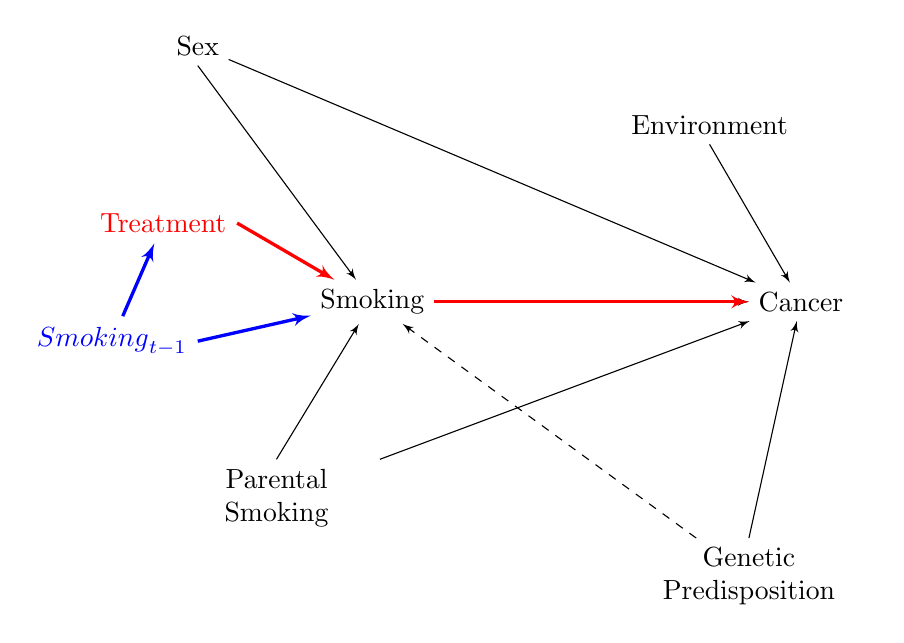
\begin{tikzpicture}[>=latex',circ/.style={draw, shape=circle, node distance=5cm, line width=1.5pt}]
    \draw[->] (0,0) node[left] (X) {Smoking} -- (4,0) node[right] (Y) {Cancer};
    \draw[->] (-3,3) node[above] (Z) {Sex} -- (X);
    \draw[->] (Z) -- (Y);
    \draw[->] (3.5,2) node[above] (A) {Environment} -- (Y);
    \draw[->] (4,-3) node[below, text width=3cm, align=center] (E) {Genetic\\Predisposition} -- (Y);
    \draw[->] (-2, -2) node[below, text width=2.5cm, align=center] (W) {Parental\\Smoking} -- (X);
    \draw[->] (W) -- (Y);
    \draw[->, dashed] (E) -- (X);
    
    \draw[->, very thick, color=red] (-2.5,1) node[left, color=red] (Tr) {Treatment} -- (X);
    \draw[->, very thick, color=red] (X) -- (Y);
    \draw<2->[->, very thick, color=blue] (-3,-0.5) node[left, color=blue] (X2) {$\text{Smoking}_{t-1}$} -- (X);
    \draw<2->[->, very thick, color=blue] (X2) -- (Tr);
\end{tikzpicture}
\end{center}
\end{frame}


\frame{

## Noncompliance analysis

Choices:

 1. Intention to treat analysis
 
 2. As-treated analysis
 
 3. Exclude noncompliant cases
 
 4. Estimate a Local Average Treatment Effect (LATE)
   - aka Compliance Average Treatment Effect (CATE)

???

Example: one-sided noncompliance in voter mobilization

Phone calls do not reach everyone in the treatment group

**How to prevent attrition?**
  - Discuss in groups
  - 1: Pretest for differential attrition rates between groups

**Example: two-sided noncompliance**

Encouragement designs: there is an existing resource that we want to encourage people to use (e.g., going to the library)
We want to know what effect library use has on childrens' educational outcomes.
We randomly send letters to some people encouraging them to go to the library
Not all of them do, so we have noncompliance
And some of those who do not receive letters go to the library, so we have noncompliance on both sides
}


\frame{

\frametitle{Noncompliance}

\begin{itemize}
\item Asymmetric (one-sided) noncompliance:
$ITT = \overline{Y}_1 - \overline{Y}_0$
$LATE = \frac{ITT}{Pct. Compliant}$
\item Symmetric (two-sided) noncompliance:
	\begin{itemize}
	\item Stronger assumptions are required to analyze it
	\item \textit{Monotonicity}
	\item This is a classic design trumps analysis problem
	\end{itemize}
\end{itemize}

}






\subsection{Issues in panel designs}
\frame{\tableofcontents[currentsubsection]}


\frame{
\frametitle{What is a panel?}

}

\frame{

\frametitle{Benefits of Panels}

\begin{itemize}\itemsep1em

\item

\end{itemize}

}

% repeated measures of outcomes (effect duration)

% repeated treatments (Druckman and Leeper 2012)



\frame{

Commercial panels

}


% custom panels (from MTurk or elsewhere)
\frame{
\frametitle{Custom Panels}
\begin{itemize}\itemsep1em
\item Creating your own panel is great
	\begin{itemize}
	\item Carefully sample on specific characteristics % stanford model; qualification model; database model
	\item Organize repeated interviewing or interaction
	\end{itemize}
\item Lots of additional issues
	\begin{itemize}
	\item Recruitment/Compensation
	\item Attrition
	\item Panel Conditioning
	\end{itemize}
\item See Callegaro et al. 2014. \textit{Online Panel Research: A Data Quality Perspective}. Wiley.
\end{itemize}
}



\frame{

\frametitle{Risks I: Recruitment}

\begin{itemize}\itemsep1em

\item

\end{itemize}

}


\frame{

\frametitle{Risks II: Attrition}

\begin{itemize}\itemsep1em

\item

\end{itemize}

}

% attrition
\frame{
\frametitle{Attrition}
\begin{itemize}\itemsep1em
\item We care about two issues:
	\begin{itemize}
	\item Who leaves a study early
	\item When they leave a study
	\end{itemize}
\item<2-> We care about representativeness (not just demographically)
\item<3-> Analyze when participants leave study to identify difficult, confusing, or problematic study elements
	\begin{itemize}
	\item Ideally, do pilot tests
	\end{itemize}
\end{itemize}

}

\frame{

Considerations:

 - Symmetric, possibly random, attrition
 
 - One-sided or systematic attrition
 
 - Pre-treatment/post-treatment
 
 - Pre-measurement/post-measurement


Statistically, as soon as one unit leaves study, it is no longer an experiment! Yet, we cannot force units to stay in an experiment.

When do we exclude cases? When do we impute missing data?

What can we do practically to prevent or respond to attrition?
 
 - Adaptive design: anticipate spending more resources on those likely to attrit
 - Pretesting: try to assess who is likely to attrit in a pilot study so you can identify where to expend resources

 - Treatment attrition versus measurement attrition
  - Measurement attrition is a missing data problem
  - Treatment attrition means we don't even know if the unit would have taken their assigned treatment
}






\frame{

\frametitle{Risks III: Panel Conditioning}

\begin{itemize}\itemsep1em

\item

\end{itemize}

}


\section{Treatment Self-Selection}
\frame{\tableofcontents[currentsection]}

\frame{

Bennett and Iyengar\footnote{Bennett, W. Lance, and Shanto Iyengar. 2008. ``A new era of minimal effects? The changing foundations of political communication.'' \textit{Journal of Communication} 58(4): 707--31.}:

\begin{quote}\small
manipulational control actually weakens the ability to generalize to the real world where exposure to politics is typically voluntary. Accordingly, it is important that experimental researchers use designs that combine manipulation with self-selection of exposure. (724)
\end{quote}

}


\frame{

Hovland\footnote{Hovland, Carl I. 1959. ``Reconciling conflicting results derived from experimental and survey studies of attitude change.'' \textit{American Psychologist} 14(1): 8--17.}:

\begin{quote}\small
It should be possible to assess what demographic and personality factors predispose one to expose oneself to particular communications and then to utilize experimental and control groups having these characteristics. Under some circumstances the evaluation could be made on only those who select themselves, with both experimental and control groups coming from the self-selected audience. (16)
\end{quote}


}




% ETHICS
\section{Research Ethics}
\frame{\tableofcontents[currentsection]}

\frame{
	\frametitle{The Belmont Report}
	
	\small
	\begin{itemize}
	\item Commissioned by the U.S. Government in 1979\footnote{\url{http://www.hhs.gov/ohrp/humansubjects/guidance/belmont.html}}
	\item Three overarching principles:
		\begin{enumerate}
		\item Respect for persons
		\item Beneficence
		\item Justice
		\end{enumerate}
	\item Three policy implications:
		\begin{itemize}
		\item Informed consent
		\item Assessment of risks/benefits
		\item Care for vulnerable populations
		\end{itemize}
	\end{itemize}

}


\frame{
	\frametitle{Informed Consent}
	\begin{itemize}
	\item Persons must consent to being a research subject
	\item<2-> What this means in practice is complicated
		\begin{itemize}
		\item What is research?
		\item What is consent?
		\item What is ``informed'' consent?
		\end{itemize}
	\item<3-> Cross-national variations
		\begin{itemize}
		\item Consent forms required in U.S.
		\item Not required in UK
		\end{itemize}
	\end{itemize}

}

\frame{
\frametitle{Benefits and Harm}
	\begin{itemize}\itemsep2em
	\item What is a ``benefit''?
	\item What is a ``harm''?
	\item How do we balance the two?
	\end{itemize}
}


\frame{
	\frametitle{Privacy}
	\begin{itemize}
	\item EU Data Protection Directive (1995) and UK Data Protection Act (1998)
	\item Deals with ``personal data''
	\item Data can be processed when:
		\begin{itemize}
		\item Consent is given
		\item Data are used for a ``legitimate'' purpose
		\item Anonymous or confidential
		\end{itemize}
	\item Data cannot leave the EU except under conditions
	\end{itemize}
}


\frame{
	\frametitle{{\normalsize Lots of Other Ethical Questions}}
	\begin{enumerate}
	\item<2-> Funding
	\item<3-> Independence and Politicization
	\item<4-> Vulnerable populations (e.g. children, sick)
	\item<5-> Cross-national research
	\item<6-> Participant-observation disclosures
	\item<7-> End uses/users of research
	\item<8-> Others?
	\end{enumerate}
}


\section{Short Presentations}
\frame{\tableofcontents[currentsection]}




\frame{
	\frametitle{Wrap-up}
	\begin{itemize}
	\item Thanks to all of you!
	\item Stay in touch (\href{mailto:t.leeper@lse.ac.uk}{t.leeper@lse.ac.uk})
	\item Good luck with your research!
	\end{itemize}
}

\appendix
\frame{}

\end{document}
